\section{Aufbau}
\label{sec:Aufbau}
Der Aufbau der Wärmepumpe zur Messung der gesuchten Kenngrößen ist in \autoref{fig:Wärmepumpe_durch} dargestellt.
Sie besteht aus zwei Reservoiren, in denen sich Wasser befindet, welches von Rührmotoren durchgerührt wird. 
Das ist wichtig, damit das Wasser eine homogene Temperatur besitzt und die von den zwei digitalen Thermometern, die sich in den Reservoiren befinden,
gemessene Temperatur keine großen Fehler aufweist.
Das System der Wärmepumpe beruht auf einer Kupferschlange die mit dem Transportgas Dichlordifluormethan (Cl$_2$F$_2$C) gefüllt ist und zu einem Kreislauf
geschlossen ist. 
In dem sich in Reservoir 2 befindlichen Teil der Kupferschlange verdampft das Transportgas und entzieht dem Wasser in Reservoir 2 
somit die Verdampfungswärme $L$.
Reservoir 2 ist somit das wärmeabgebende, kältere Reservoir.
Es folgt eine Steuerungsvorrichtung, die gewährleistet, dass flüssige Überreste im Gas zerstört werden, sodass nur Dampf vorhanden ist.
Anschließend durchläuft der Dampf den Kompressor und wird dort nahezu adiabatisch komprimiert und somit stark erhitzt.
Der Druck wird dadurch soweit erhöht, dass sich das Transportgas in der Kupferschlange im Reservoir 1 wieder verflüssigt.
Währenddessen gibt das Transportgas die Kondensationswärme $L$ an das Wasser im Reservoir ab und erhitzt es. Reservoir 1 ist somit das wärmeaufnehmende,
wärmere Reservoir.
Nach dem Reservoir wird der Druck $p_b$ durch ein Barometer gemessen. 
Anschließend fließt das flüssige Transportgas durch einen Reiniger, der die Flüssigkeit von Gasresten trennt, damit im Folgenden das Drosselventil nicht beschädigt wird.
Das Drosselventil ist mit einer Steuerungsvorrichtung vor dem Kompressor verbunden und regelt die Flüssigkeitszufuhr zum 2. Reservoir in Abhängigkeit
von der Temperaturdifferenz vor und hinter dem Reservoir 2. Somit sorgt das Drosselventil mit dafür, dass nur das Transportmedium nur in Gasform in den
Kompressor gelangt.
Nach dem Drosselventil wird der Druck $p_a$ gemessen und das flüssige Transportmedium wird wieder durch das Reservoir 2 geleitet, der Kreislauf beginnt erneut.
Außerdem ist der Kompressor an ein Wattmeter angeschlossen, welches dessen elektrische Leistungsaufnahme misst.
\begin{figure}[H]
    \centering
    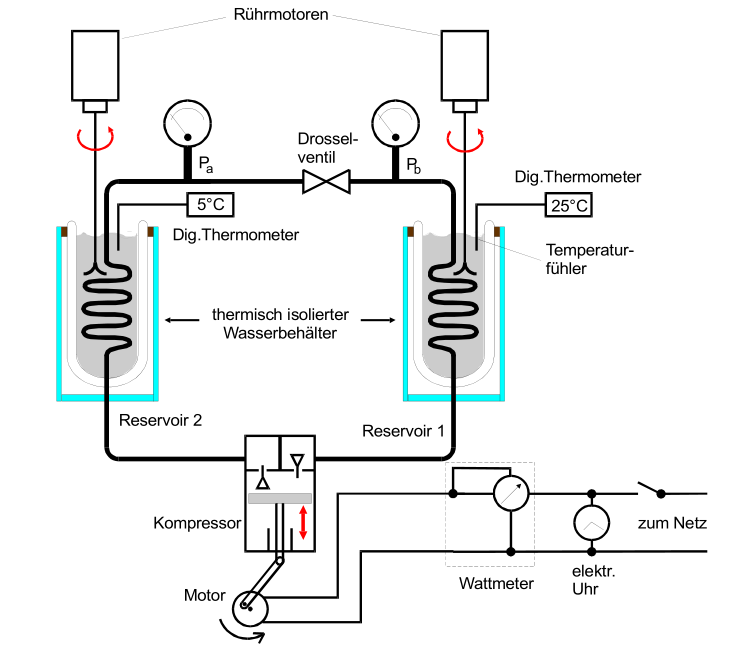
\includegraphics[width=0.6\textwidth]{build/Abb2.png}
    \caption{Schematische Darstellung der kompletten Messapparatur \cite[197]{V206}.}
    \label{fig:Wärmepumpe_durch}
\end{figure}
\section{Durchführung}
\label{sec:Durchführung}

Die Reservoire werden beide mit jeweils der gleichen Menge Wasser befüllt.
Die Thermometer und die Rührmotoren werden angeschaltet und die Anfangswerte ohne Kompressor werden abgelesen und in eine Tabelle geschrieben.
Anschließend wird der Kompressor angeschaltet und die Messung beginnt.
Es werden nun jede Minute die Werte für die Temperaturen $T_1$ und $T_2$, die Drücke $p_a$ und $p_b$ und die elektrische Leistungsaufnahme
des Kompressors $N$ abgelesen und in die Tabelle notiert. Die Messung geht solange bis $T_1$ eine Temperatur von mindestens $\qty{50}{\degree}$ erreicht.
